\section{Introduction}
\label{sec:introduction}

% state the learning objective
The objective of this laboratory assignment is to study a circuit containing an independent voltage source $V_a$, a dependent voltage source $V_c$, an a independent current source $I_d$, a dependent current source $I_b$ and seven resistors $R$. The given circuit is composed by four elementary meshes. The circuit can be seen in Figure~\ref{fig:t1_circuit}.


In Section~\ref{sec:analysis}, a theoretical analysis of the circuit is
presented. In Section~\ref{sec:simulation}, the circuit is analysed by
simulation, and the results are compared to the theoretical results obtained in
Section~\ref{sec:analysis}. The conclusions of this study are outlined in
Section~\ref{sec:conclusion}.

\begin{figure}[h] \centering
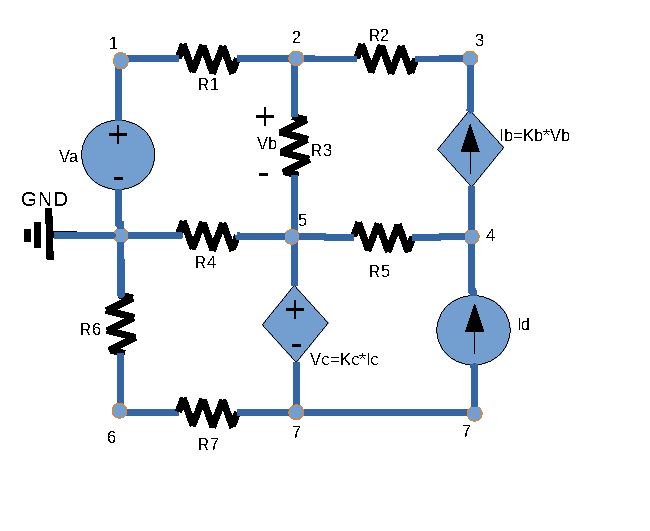
\includegraphics[width=0.6\linewidth]{t1_circuit.pdf}
\caption{Circuit with independent sources, dependent sources and resistors.}
\label{fig:t1_circuit}
\end{figure}


